\documentclass[]{article}

\usepackage[utf8]{inputenc}
\usepackage{amsmath}
\usepackage{amssymb}
\usepackage{amsthm}
\usepackage{amsfonts}
\usepackage{graphicx}
\usepackage{capt-of}
\usepackage{listings}
\usepackage{siunitx}
\usepackage[section]{placeins}
\usepackage{color} %red, green, blue, yellow, cyan, magenta, black, white
\usepackage{float}

\definecolor{mygreen}{RGB}{28,172,0} % color values Red, Green, Blue
\definecolor{mylilas}{RGB}{170,55,241}
\lstset{language=Matlab,%
    breaklines=true,%
    morekeywords={matlab2tikz},
    keywordstyle=\color{blue},%
    morekeywords=[2]{1}, keywordstyle=[2]{\color{black}},
    identifierstyle=\color{black},%
    stringstyle=\color{mylilas},
    commentstyle=\color{mygreen},%
    showstringspaces=false,%without this there will be a symbol in the places where there is a space
    numbers=left,%
    numberstyle={\tiny \color{black}},% size of the numbers
    numbersep=9pt, % this defines how far the numbers are from the text
    emph=[1]{for, end, break}\emphstyle=[1]\color{red}, %some words to emphasise
}




% Oppgavenummerering %
\renewcommand\thesection{Task \arabic{section}}
\renewcommand\thesubsection{\alph{subsection})}

% Bevis
\newcommand\TombStone{\rule{.5em}{.5em}}
\renewcommand\qedsymbol{\TombStone}
\renewcommand{\proofname}{Bevis.} % Norske bevis

\title{}
\author{Sigurd Totland | MTTK}

\begin{document}
\maketitle

\section{}
\subsection{}
We implement the functions from the textbook. The matlab code for this is shown in listing \ref{lst:reduce_gauss_mix} below.
\begin{lstlisting}[label={lst:reduce_gauss_mix}, caption={reduceGaussMix.m}]
function [xmix, Pmix] = reduceGaussMix(w, x, P)
    w = w(:);
    M = numel(w);
    n = size(x, 1);

    %% implementation
    % allocate
    xmix = zeros(n, 1);
    Pmix = zeros(n, n);

    % mean
    for i = 1:M
        xmix = xmix + w(i) * x(1:n,i);
    end

    % spread of the innovations
    P_squiggle = zeros(n,n);
    for i = 1:M
        P_squiggle = P_squiggle + w(i) * x(1:n,i) * x(1:n,i)';
    end
    P_squiggle = P_squiggle - xmix * xmix';

    % covariance
    for i = 1:M
        Pmix = Pmix + w(i) * P(:, :, i);
    end
    Pmix = Pmix + P_squiggle;
end
\end{lstlisting}

\subsection{}
What we wish to do in this problem is combine two of the components with moment matching, i.e. create a new Gaussian with moments (expectation and variance) matching that of the mixture of the two initial components. I would choose the components to combine that are as similar as possible in their moments. So for the first list, I would combine 1 and 2, obtaining $\bar \mu = 1$ and $\bar \sigma = 2$. For the second, I would combine also combine 1 and 2 obtaining $\bar \mu = 1.6$ and $\bar \sigma = 1.64$. From the script we also see that this combination is the one that looses the least of the tails of the original distribution, which is important. For the third, 2 and 3 are the best candidates for combination, because they have the same variance, and not much more of a difference in mean. The moments for this gaussian become $\bar \mu = 3.25$ and $\bar \sigma = 3.0625$. For the last one, we have two choices, either combine the two first components, which have identical mean, or the two last, having identical variance. It is evident from figure \ref{fig:combinations} that combining 2 and 3 would be a good idea in this case, our second alternative, 1 and 2 is also good, but it puts a little less emphasis on the mean, so 1 and 3 is a little more accurate. For this we get $\bar \mu = 1.25$ and $\bar \sigma = 3.0625$.

\begin{figure}[H]
\centering
\label{fig:combinations}
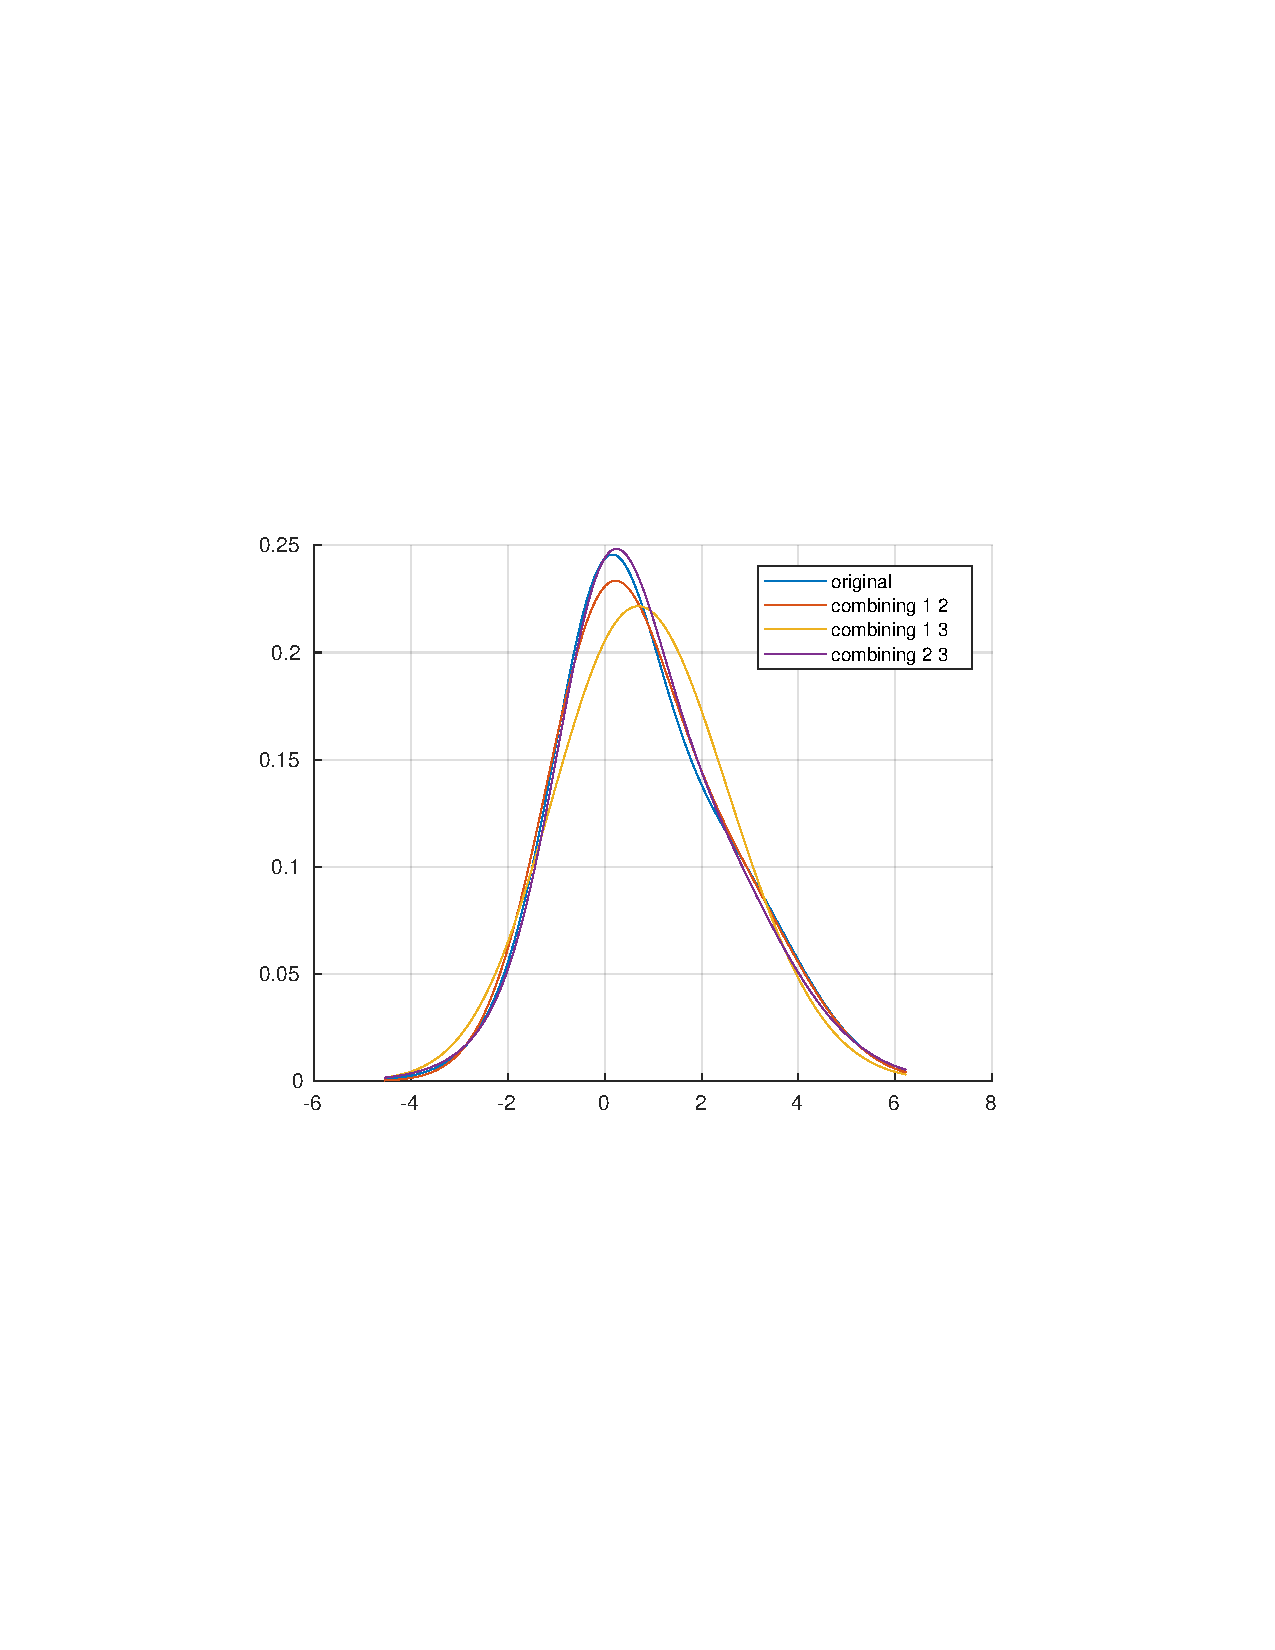
\includegraphics[width=0.3\textwidth, trim={8cm, 8cm, 8cm, 8cm, clip}]{matlab/combinations1b.pdf}
\caption{Combination choices for the fourth list}
\end{figure}

\section{}
\subsection{}
We have
\begin{equation}\begin{aligned}
\label{eq:imm_ml}
p(z_k | z_{1:k-1}) = \sum_{s_k}\int p(z_k | x_k, s_k) p(x_k | s_k, z_{1:k-1}) \Pr(s_k | z_{1:k-1})dx_k.
\end{aligned}\end{equation}
Using that the mode-conditional likelyhood is
\begin{equation}\begin{aligned}
\Lambda^{(s_k)}_k &= \int p(z_k | x_k) p(x_k | s_k, z_{1:k-1})dx_k \\
&= \int p(z_k | x_k, s_k) p(x_k | s_k, z_{1:k-1})dx_k,
\end{aligned}\end{equation}
where we have used that $p(z_k | x_k) = p(z_k | x_k, s_k)$ and inserting this into \eqref{eq:imm_ml}, we get an expression for the IMM measuerement likelyhood expressed with this and the mode probability $p_k^{(s_k)} = \Pr(s_k | z_{1:k})$ that is
\begin{equation}\begin{aligned}
p(z_k | z_{1:k-1}) = \sum_{s_k}\Lambda_k^{(s_k)}p_k^{(s_k)}.
\end{aligned}\end{equation}

\subsection{}
Using the total probability theorem we get
\begin{equation}\begin{aligned}
p(z_k | z_{1:k-1})
&= \int p(z_k | x_k, z_{1:k-1}) p(x_k | z_{1:k-1})dx_k \\
&= \int p(z_k | x_k) p(x_k | z_{1:k-1})dx_k
\end{aligned}\end{equation}
where we have used the markov assumption to obtain the second line. If we then insert the given distribution $p(x_k | z_{1:k-1}) \approx \sum_{i=1}^{N}w^i_k \delta(x_k - x_k^i)$, we get
\begin{equation}\begin{aligned}
p(z_k | z_{1:k-1})
&= \int p(z_k|x_k)  \sum_{i=1}^{N}w^i_k \delta(x_k - x_k^i) dx_k \\
&= \sum_{i=1}^{N}w^i_k p(z_k | x_k^i)
\end{aligned}\end{equation}
because of the fundamental property of the dirac delta function.

\section{}
\subsection{}
\begin{lstlisting}[caption={IMM Step 1}]
function [spredprobs, smixprobs] = mixProbabilities(obj, sprobs)
   % IMM: step 1
   %
   % sprobs (M x 1): probabilities that we are in each mode
   %
   % spredprobs (M x 1): predicted mode probabilities
   % smixprobs (M x M): mixing probabilities

   % Joint probability for this model and next
   spsjointprobs = obj.PI .* (ones(obj.M,1) *sprobs');%

   % marginal probability for next model (sum over all modes)
   spredprobs = spsjointprobs * ones(obj.M,1);% ... (6.32)?

   % conditionional probability for model at this time step on the next.
   smixprobs =spsjointprobs ./ (spredprobs * ones(1, obj.M)); % ... (6.26)?
end
\end{lstlisting}

\subsection{}
\begin{lstlisting}[caption={IMM Step 2}]
function [xmix, Pmix] = mixStates(obj, smixprobs, x, P)
   % IMM: step 2
   % smixprob (M x M): mixing probabilities
   % x (dim(state) x M): means to mix
   % P (dim(state) x dim(state) x M): covariances to mix
   %
   % xmix (dim(state) x M): mixed means
   % Pmix (dim(state) x dim(state) x M): mixed covariances

   % allocate
   xmix = zeros(size(x));
   Pmix = zeros(size(P));

   % one gaussian for each row
   for i = 1:obj.M
       xmix(i) = reduceGaussMix(smixprobs(i), x(i), P(i));
   end
end
\end{lstlisting}

\subsection{}
\begin{lstlisting}[caption={IMM Step 3}]
function [xpred, Ppred] = modeMatchedPrediction(obj, x, P, Ts)
   % IMM: prediction part of step 3
   % x (dim(state) x M matrix): mean to predict
   % P (dim(state) x dim(state) x M): covariance to predict
   % Ts: sampling time for prediction.
   %
   % xpred (dim(state) x M): predicted means
   % Ppred (dim(state) x dim(state) x M): predicted covariances

   % allocate
   xpred = zeros(size(x));
   Ppred = zeros(size(P));

   % mode matched prediction
   for i = 1:obj.M
       [xpred(i), Ppred(i)] = predict(obj.modelFilters(i), x(i), P(i), Ts);
   end
end
\end{lstlisting}

\end{document}

